\documentclass[../manuale_sviluppatore.tex]{subfiles}

\begin{document}

\subsection{Pattern architetturale: MVP}
Il pattern architetturale scelto è il \emph{Model View Presenter}. 
Il model è un'interfaccia che definisce i dati da visualizzare o su cui agire nell'interfaccia utente; farà inoltre i calcoli necessari, ad esempio la \emph{Distance Matrix}.
La view è un'interfaccia che visualizza i dati e indirizza i comandi dell'utente (eventi) al presenter per agire su quei dati.
Il presenter agisce sul model e sulla view. Recupera i dati e li formatta per la visualizzazione.\\
Nella specifico nella nostra architettura sono presenti diversi componenti appartenenti a tale formato, e verranno descritti più nel dettaglio di seguito.\\
Nella nostra architettura le componenti hanno il presenter e la view, non hanno un modello perchè non ci saranno calcoli bensì eventi da aggiornare. Nel caso dei
grafici la view viene realizzata tramite le funzionalità di D3.

\subsection{Architettura di dettaglio}
\subsubsection{Il client}

\begin{figure}[H]
	\centering
	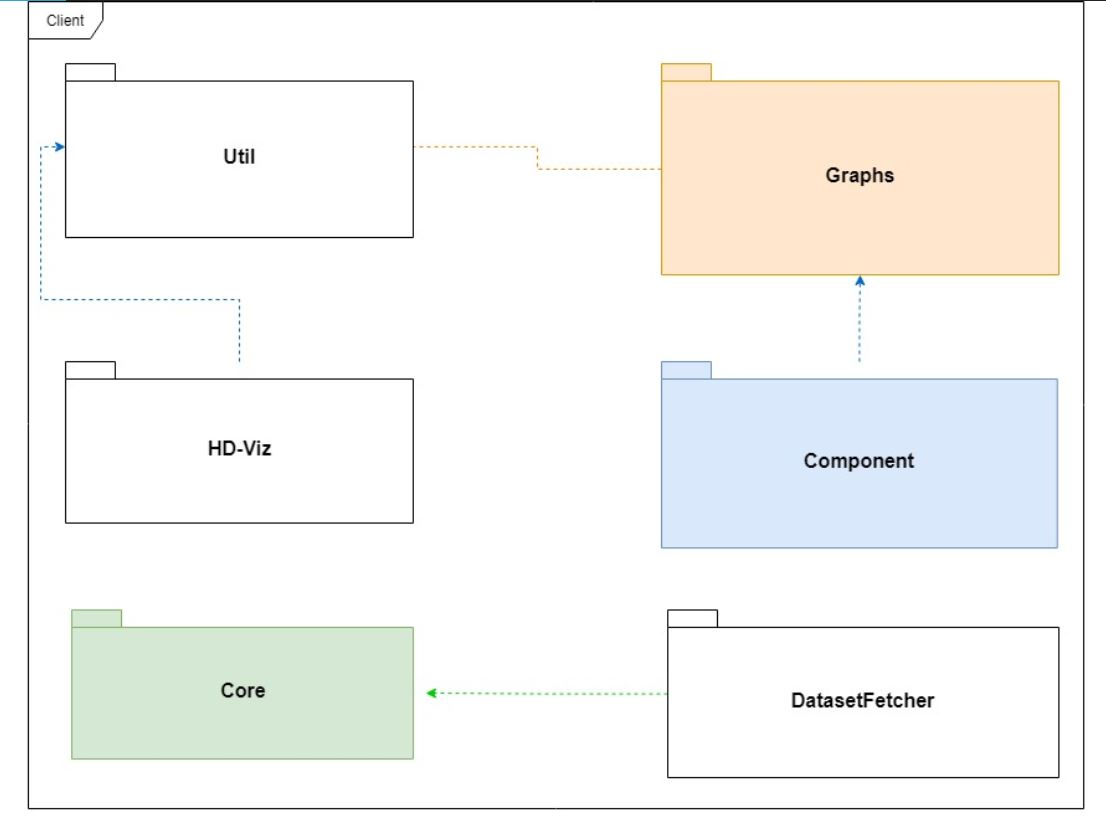
\includegraphics[width=18cm]{img/core.jpg}
	\caption{Introduzione a Hd-Viz}
\end{figure}

\emph{HD Viz manager} è il core dell'architettura, si delegherà la visualizzazione ai vari Manager, inoltre terrà traccia 
dei dati per evitare istanze multiple del Dataset, della DistanceMap e dei grafici una volta creati. Nel momento in cui 
verrà modificato il dataset per modificare le visualizzazioni, farà da tramite creando una copia del dataset originale e usando
tali copie per le modifiche, cosicchè il dataset originale resti invariato.
Collaborerà poi assieme al \emph{GraphCreatorManager} che gestirà le factories per i vari modelli dei grafici. 
Il \emph{CurrentGraphManager} verificherà se le factories saranno in grado di costruire il grafico, quindi comunicherà con il 
presenter e il modello del grafico relativo. \\


\begin{figure}[H]
	\centering
	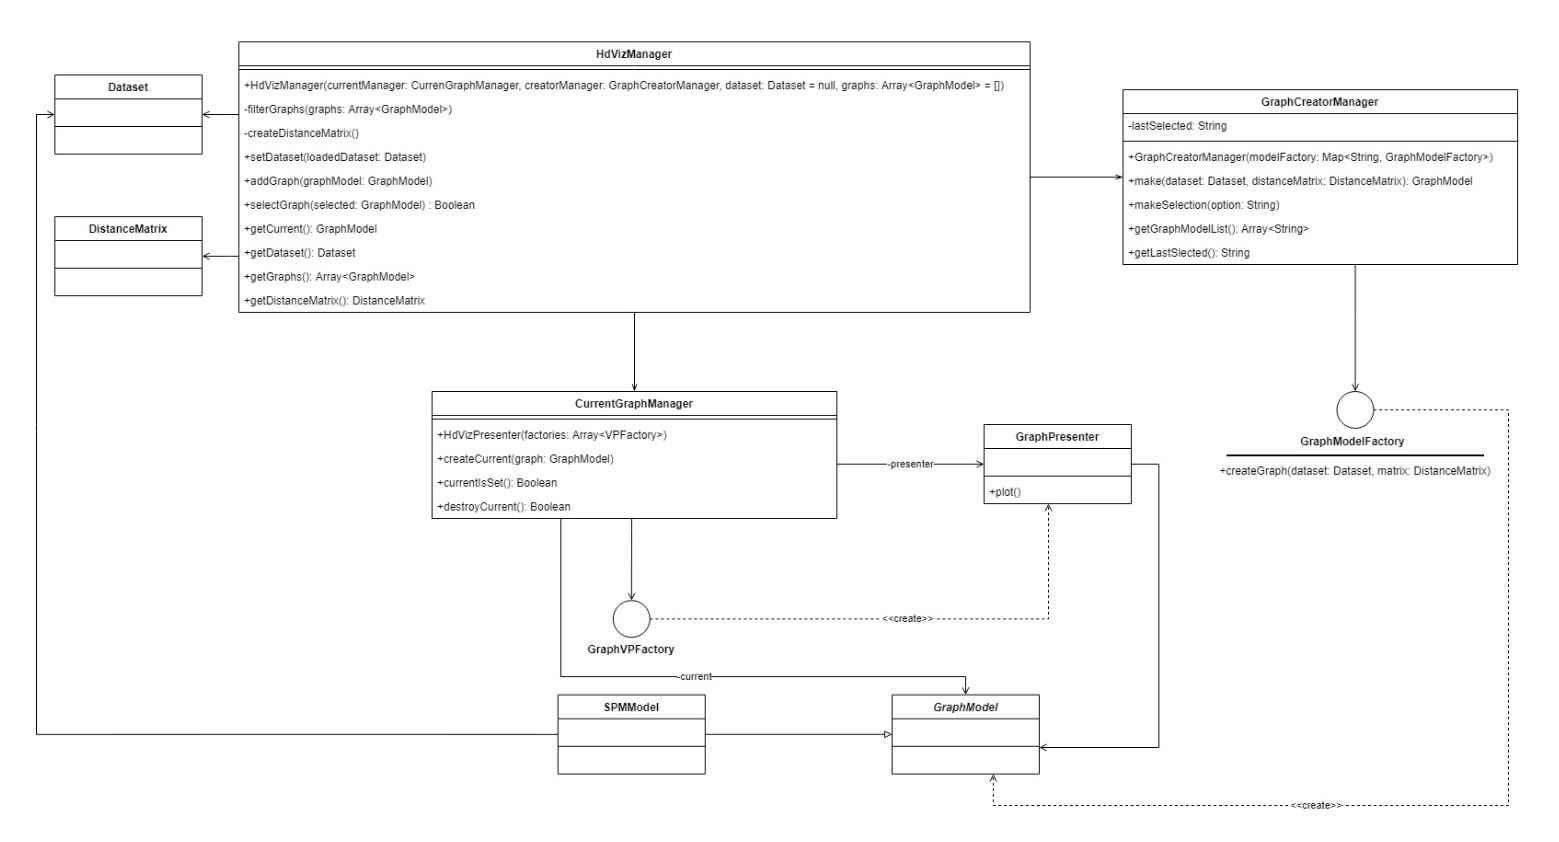
\includegraphics[width=18cm]{img/core-hdvizmanager.jpg}
	\caption{HD-Viz Manager}
\end{figure}

Graphs contiene le diverse visualizzazioni che la nostra applicazione metterà a disposizione, Component mette a disposizione una serie di componenti che permettono di aggiungere funzionalità ai grafici.
Questi ultimi modificano le proprietà di visualizzazione dei grafici, dialogando con modelli tramite interfacce. Ciascun component ha un \emph{Presenter} che gestisce la logica e la \emph{View} che renderizza il tutto,
infatti tramite le interfacce ogni grafico implementerà dimensioni e colori a modo proprio.

\begin{figure}[H]
	\centering
	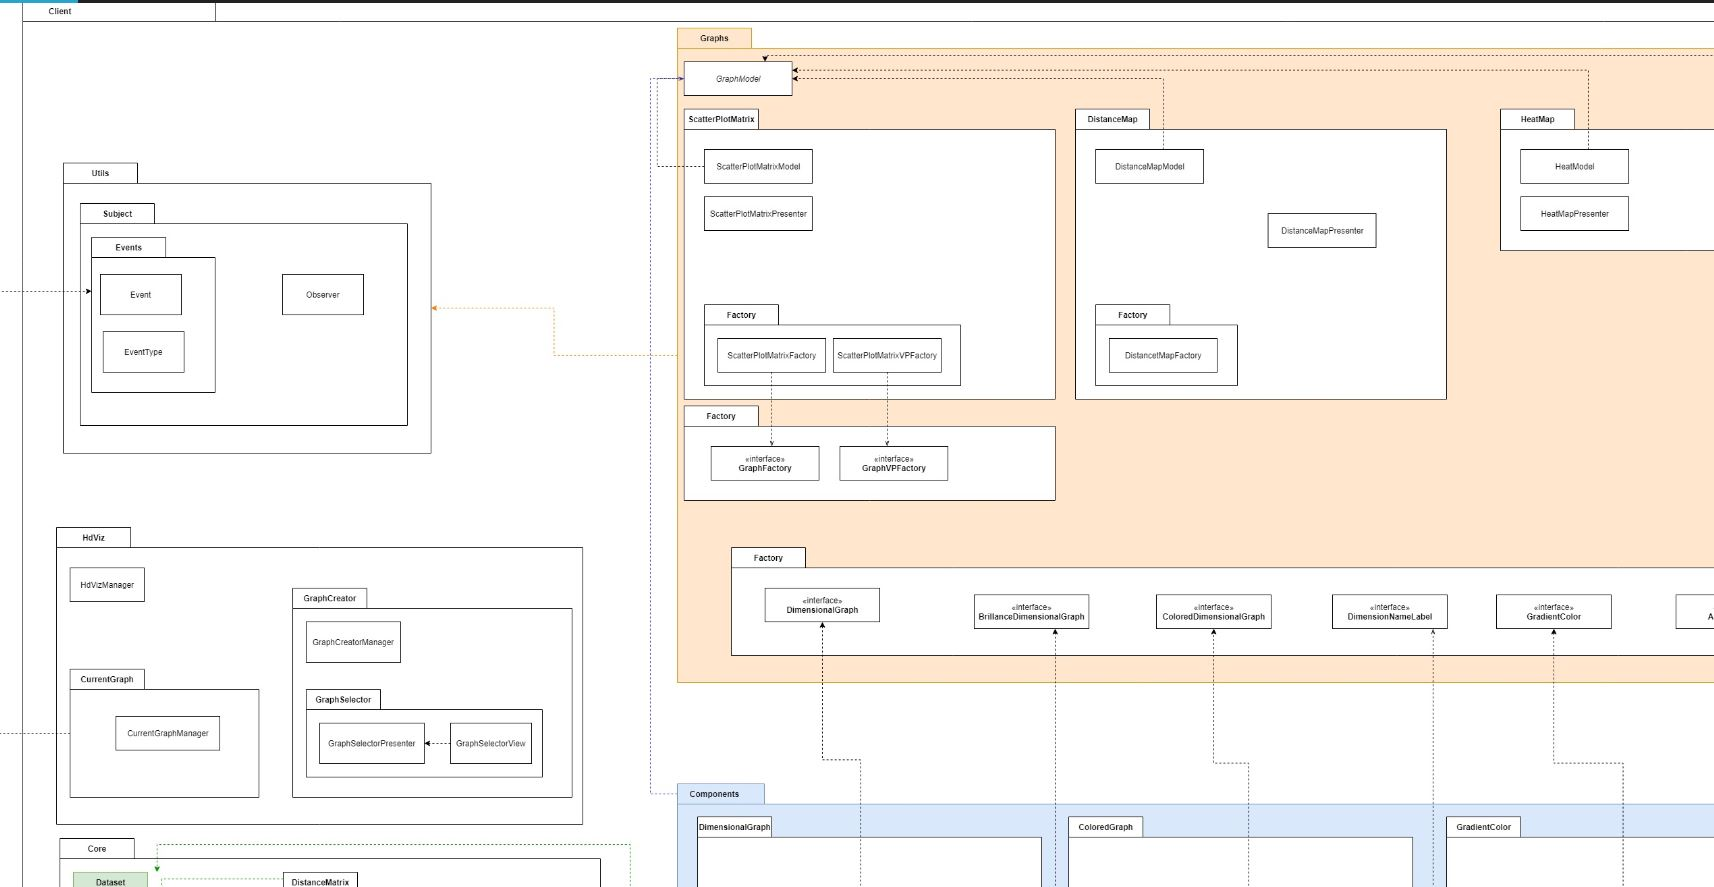
\includegraphics[width=18cm]{img/graph-e-hdviz.jpg}
	\caption{Relazioni tra graph e HD-Viz}
\end{figure}


Ciascun grafico eredita il \emph{GraphModel}; dentro il modello salverà le impostazioni del grafico, ad esempio il gradiente colori, il dataset, i label delle righe ecc.

\begin{figure}[H]
	\centering
	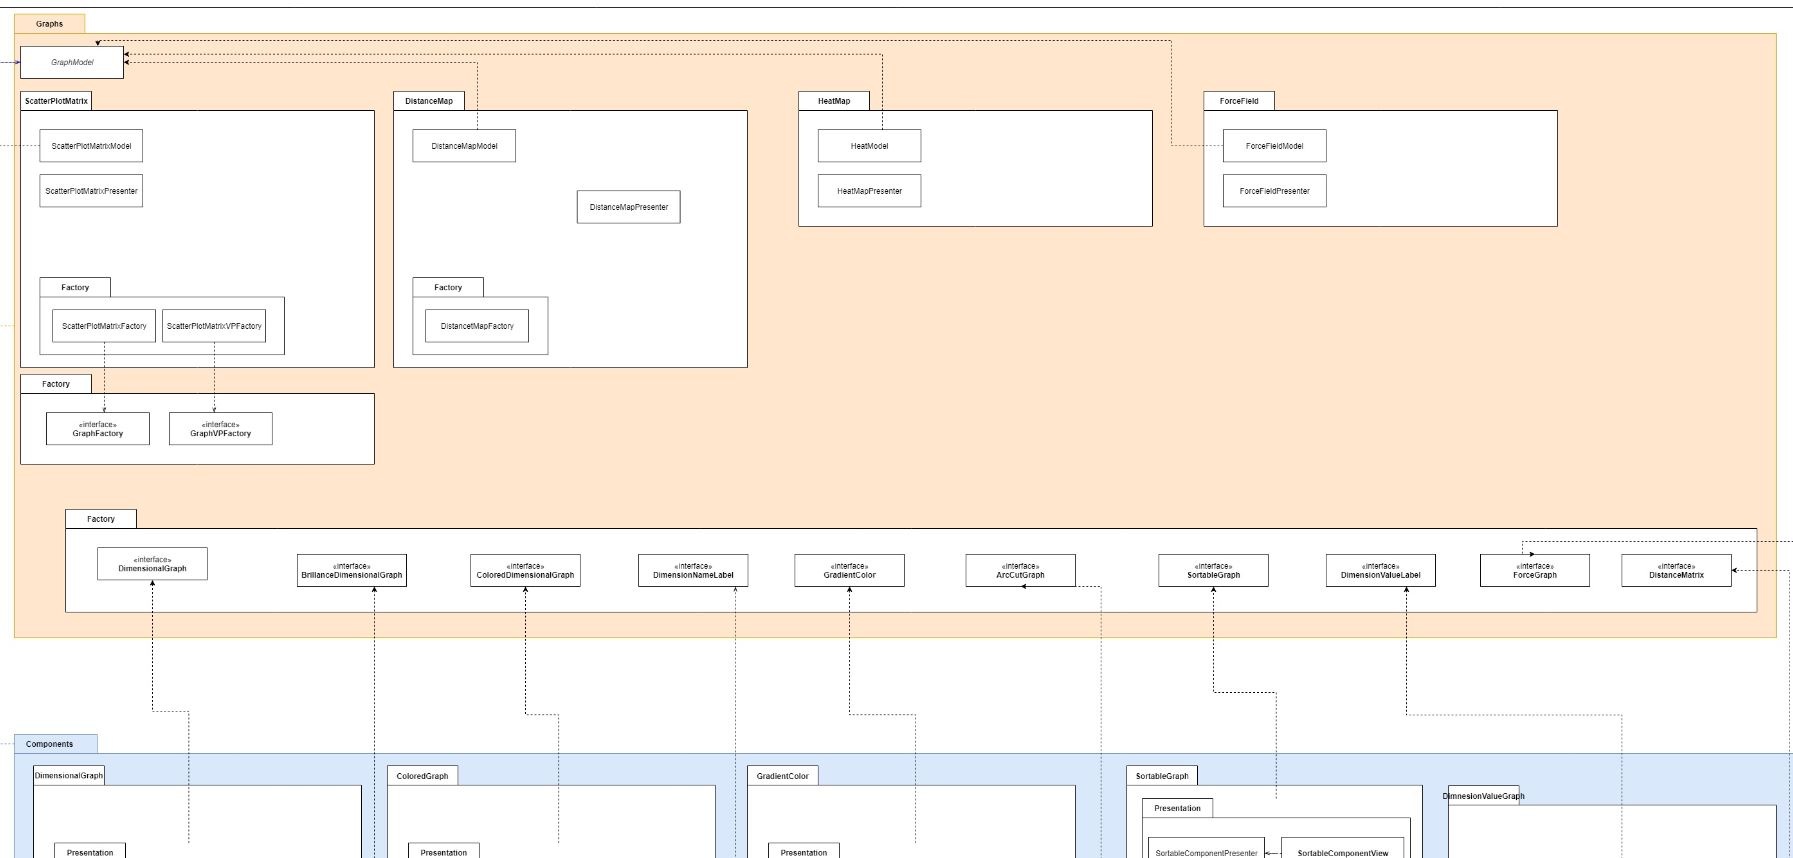
\includegraphics[width=18cm]{img/graphs-e-components.jpg}
	\caption{Relazioni tra graphs e components}
\end{figure}


Collegando il model al presenter, i vari componenti che modificano la visualizzazione notificheranno il presenter; a sua volte modificherà il model, il quale si aggiornerà di conseguenza, 
e notificherà al presenter dei cambiamenti.
Ciò avverrà tramite i metodi update. In particolare verrà aggiornato l'EventType.

\subsubsection{Il server}

Il lato server è stato realizzato con \emph{Express}, il quale si occuperà di gestire la sessione per collegarsi al server.
SQLApplication si occuperà di caricare la configurazione, che verrà passata ad SQLRoute.\\
Configuration e ConfigurationController si occuperanno di raccogliere le informazioni relative alla connessione con un database, la quale verrà stabilita tramite un file
json dove vi sarà presente la query.\\
MDataset (MinimalDataset) controllerà che il dataset passato sia valido perchè potrebbero esserci oggetti che non possono essere rappresentati. Successivamente
CSVApplication si occuperà di creare un file JSON che contenga i dati letti, se il file è corretto, allora CSVRuoute risponderà positivamente.

\begin{figure}[H]
	\centering
	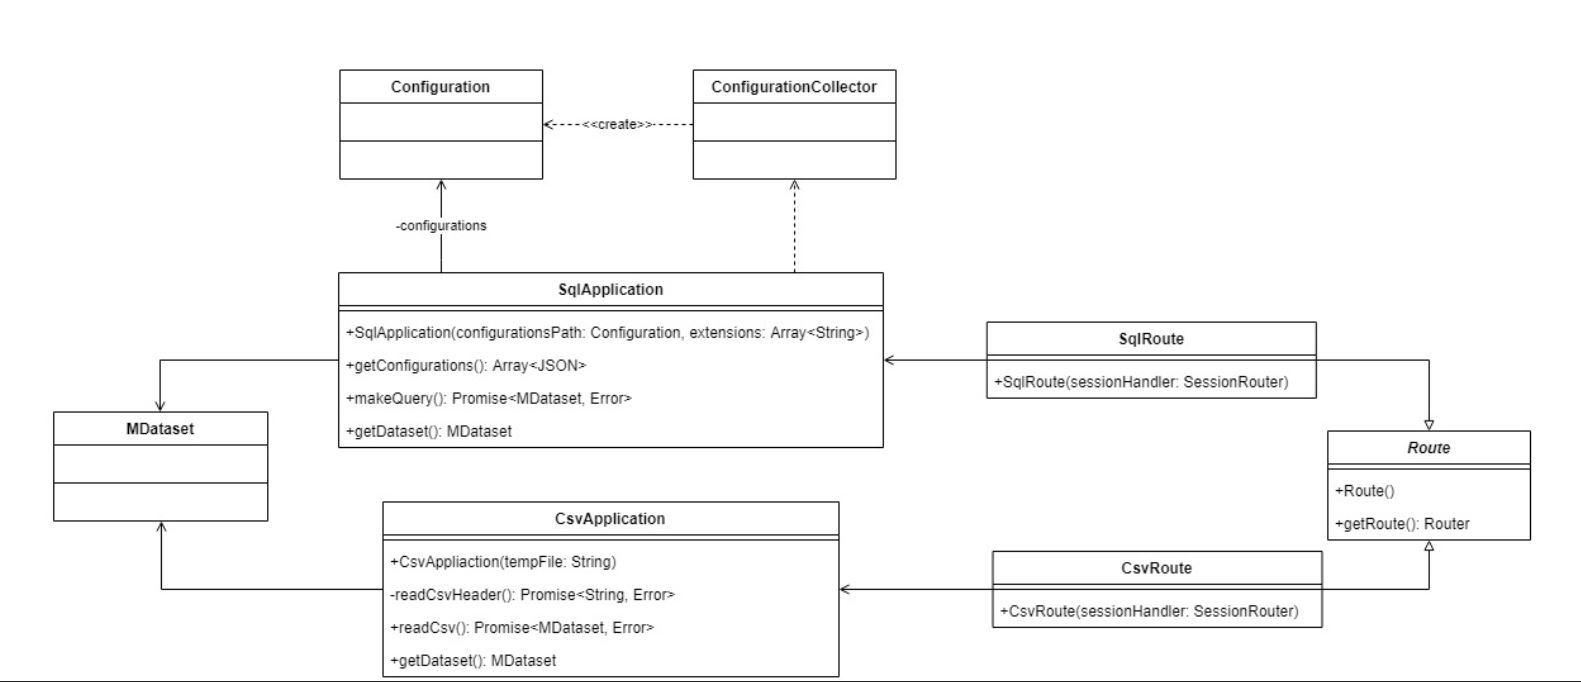
\includegraphics[width=18cm]{img/server.jpg}
	\caption{Server HD-Viz}
\end{figure}

\end{document}